\documentclass[11pt,a4paper]{report}
\usepackage{minted} %must be installed
\usepackage{mathtools} % misc math 
\usepackage{amssymb} % math symbols
\usepackage[utf8]{inputenc}
\usepackage[T1]{fontenc}
\usepackage{enumitem} % for [leftmargin=*]
\usepackage{geometry} % for better controll of margins

\usepackage[romanian]{babel} %romanian names

\usepackage[dvipsnames]{xcolor}
\usepackage{hyperref}
\hypersetup{colorlinks=true, linkcolor=cyan, citecolor=green, filecolor=black, urlcolor=blue}


\usepackage{tikz}
\usetikzlibrary{arrows}
\usepackage{hyperref}

\usepackage{sectsty}
\chaptertitlefont{\centering\LARGE}
\sectionfont{\Large}

\geometry{a4paper,left=25mm,right=20mm,top=20mm,bottom=30mm}

\author{Pavel Andrei}
\date{}
\title{Portofoliu Structuri de date}

%\AtBeginEnviroment{enumerate}{}

%\usepackage{datatool} %for putting files and outputs

%\newcommand{\code}{\}
\newminted[cpp]{cpp} {
  linenos,
  frame=single,
  %breaklines,
  %style=vs,
  fontsize=\large,
  escapeinside=@@
}
\newcommand{\cppcode}[1]{\input{cpp_latex/#1}}

\usepackage{xparse}

\DeclareDocumentEnvironment{problema}{O {1} o}{
  \begin{enumerate}[leftmargin=*]
    \addtocounter{enumi}{#1}
    \addtocounter{enumi}{-1}
    \item
}{
  \end{enumerate}
  \IfValueT{#2}{
    \cppcode{#2}
  }
}

%\newcommand{\problemaArg}{} % dummy macro
% \DeclareDocumentEnviroment{problema}{O {1} m}{
  % %\renewcommand{problemaArg}{HI}
  % \begin{enumerate}[leftmargin=*]
    % \addtocounter{enumi}{#1}
    % \addtocounter{enumi}{-1}
    % \item
% }{
% \end{enumerate}
% #2
%}


\newcommand{\mat}[1]{\mathcal{M}_{#1}(\mathbb{R})}
\newcommand{\matmn}{\mat{m\times{}n}}
\newcommand{\matn}{\mat{n}}

\usepackage{tocloft}

\renewcommand{\cftchapleader}{\cftdotfill{\cftdotsep}}
%\hypersetup{colorlinks=true, linkcolor=cyan, citecolor=green, filecolor=black,urlcolor=blue}

\newcommand{\lab}[1]{
  %\section*{Laborator #1}
  %\addcontentsline{toc}{section}{Laborator #1}
}
\newcommand{\labtitle}[2]{
  \chapter*{#1}
  \addcontentsline{toc}{chapter}{#2}
}
\newcommand{\commonFile}[2]{
  \subsection*{\texttt{#1}}
  \label{#2}
  \addcontentsline{toc}{section}{#1}
  \cppcode{src/#1}
}

\begin{document}
\tableofcontents
\pagebreak

\labtitle{Fișiere comume}{Fișiere comune}
\commonFile{utils.h}{utilsh}
\commonFile{matrix.h}{matrixh}
\commonFile{vector.h}{vectorh}
\commonFile{stack.h}{stackh}
\commonFile{queue.h}{queueh}
\commonFile{list.h}{listh}
\commonFile{doubleList.h}{doubleListh}
\commonFile{graphEdgeList.h}{graphEdgeListh}
\commonFile{graphAdjacencyList.h}{graphAdjacencyListh}
\commonFile{ptrRange.h}{ptrRangeh}
\commonFile{dirGraphMat.h}{dirGraphMath}
\commonFile{dirGraphAdjacencyList.h}{dirGraphAdjacencyListh}
\commonFile{weightedDirGraphMat.h}{weightedDirGraphMath}

\labtitle{Alocarea dinamică a memoriei.\\ Tipuri specifice.}{Alocarea dinamica a memoriei. Tipuri specifice.}
% \maketitle
\lab{1}
  \begin{problema}[16][src/lab1_16_matrix.cpp]
    Scrieți funcții pentru implemetarea operațiilor specifice pe matrice de numere reale cu $m$ linii și $n$ coloane:
    suma, diferența și produsul al două matrice, produsul dintre o matrice și un scalar real, transpusa unei matrice, norme matriceale specifice\footnote{
      Dacă $A \in \matmn$, atunci
      $||A||_1 = \max\limits_{1\leq j \leq n} \sum\limits_{i=1}^m |a_{ij}|$,
      $||A||_\infty = \max\limits_{1 \leq i \leq m} \sum\limits_{j=1}^{n}|a_{ij}|$,
      $||A||_{F} = \sqrt{\sum\limits_{i=1}^{m} \sum\limits_{j=1}^{n} a_{ij}^{2} }$.
    },
    citirea de la tastatură a componentelor unei matrice, afișarea componentelor matricei.
    Pentru cazul particular al unei matrice patratice de ordin $n$, să se testeze dacă aceasta satisface criteriul de dominanță pe linii\footnote{
      $A \in \matn$ este strict diagonal dominantă pe linii dacă
      $|a_{ii}| > \sum\limits_{
        \substack{
          j = 1 \\
          j \ne i
        }
      }^{n}
      |a_{ij}|$, pentru orice $i = 1,...,n$.
    } sau pe coloane\footnote{
      $A \in \matn$ este strict diagonal dominantă pe colonane dacă
      $|a_{jj}| > \sum\limits_{
        \substack{
          i = 1 \\
          i \ne j
        }
      }^{n}
      |a_{ij}|$, pentru orice $j = 1,...,n$.
    }.
    Se vor folosi tablouri bidimensionale alocate static.
  
  \end{problema}
  %\cppcode{src/lab1_16_matrix.cpp}
\lab{2}
  \begin{problema}[18][src/lab2_18_vector.cpp]
  Scrieți funcții pentru implementarea operațiilor specifice pe vectori din $\mathbb{R}^n$: suma, diferența și produsul scalar al doi vectori,
  produsul dintre un vector și un scalar real, negativarea unui vector, norma euclidiană a unui vector,
  citirea de la tastură a celor $n$ componente ale unui vector, afișarea componentelor vectorului sub forma unui $n$-uplu de elemente.
  Se vor folosi tablouri unidimensionale alocate dinamic.
\end{problema}


\labtitle{Tablouri}{Tablouri}
\lab{3}
%\begin{problema}[6][src/lab3_06_punct.cpp]
  %Definiți în C++ un nou tip de dată corespunzător noțiunilor de punct în plan,
  %tip de dată ce va fi denumit \texttt{Punct2D}.
  %\begin{enumerate}[label=\alph*)]
  %\item Scrieți funcții pentru: calculul distanței dintre două astfel de puncte,
    %citirea de pa tastatură și afișarea unei date de tip \texttt{Punct2D}
  %\item Citiți de la tastatură $n$ date de tip \texttt{Punct2D} și, de asemenea,
    %un punct fix $A(a, b)$. Afișați punctele cele mai apropiate și cele mai
    %depărtate de punctul fix $A$ (alocare dimamică).
    %\item Testați dacă toate cele $n$ puncte citie sunt egal depărtate de punctul fix $A$.
    %\item Eliminați punctele cu abcisa sau ordonata negativă din șirul celor $n$ puncte
      %citite de la tastatură (alocare dinamică).
    %\item Dându-se 3 puncte distincte din plan, verificați dacă punctele sunt
      %sau nu coliniare\footnote{
        %Punctele $A(x_A, y_A),\ B(x_B, y_A),\ C(x_C, y_C)$ sunt coliniare
        %$\iff \left|
          %\begin{matrix}
            %x_A & y_A & 1\\
            %x_B & y_B & 1\\
            %x_C & y_C & 1\\
          %\end{matrix}
        %\right| = 0$
      %}. În cazul în care punctele sunt necoliniare, afișați centrul și
      %raza cercului determinat în mod unic de cele 3 puncte\footnote{
        %Dacă punctele $A(x_A, y_A),\ B(x_B, y_A),\ C(x_C, y_C)$ sunt necoliniare,
        %cercul determinat în mod unic de acestea are raza $R = abc/(4S)$,
        %unde $a, b, c$ sunt lungimile laturilor $\Delta\text{-ului }ABC$,
        %iar $S$ este aria acestuia, iar centrul cercului este $O(x_O, y_O)$,
        %cu $x_O = \left[ (x^2_A+y^2_A)(y_B-y_C) +
          %(x^2_B + y^2_B)(y_C-y_A) +
          %(x^2_C+y^2_C) (y_A-y_B) \right]/D $,
        %$y_O = \left[ (x^2_A+y^2_A)(x_C-x_B) +
          %(x^2_B + y^2_B)(x_A-x_C) +
          %(x^2_C+y^2_C) (x_B-x_A) \right]/D $, și
        %$D = 2[x_A(y_B - y_C) + x_B(y_C-y_A) +x_C (y_A-y_B) ] $.
       % 
      %}.
  %\end{enumerate}
  % \end{problema}
\begin{problema}[7][src/lab3_07_system.cpp]
  Folosind structurile de date \texttt{VECTOR} și \texttt{MATRICE} definite la curs și funcțiile necesare,
  rezolvați următorul sistem algebric liniar cu $n$ ecuații și $n$ necunoscute folosind metoda lui Gauß de eliminare.

  \begin{equation*}
    \left\{
    \begin{aligned}
      2x_1 - x_2 &= 1\\
      -x_1 + 2x_2 - x_3 &= 1\\
      -x_2 + 2x_3 - x_4 &= 1\\
      \cdots\cdots\cdots\cdots &\\
      -x_{n-2} + 2x_{n-1}-x_n &= 1\\
      -x_{n-1} + 2x_n &= 1, \hspace{0.5cm} n \in \mathbb{N}, 2 \leq n \leq 50
    \end{aligned}.
  \right.
  \end{equation*}
\end{problema}

\labtitle{Liste liniare simplu înlănțuite \\ Stive și cozi}{Liste liniare simplu înlănțuite. Stive și cozi}
\lab{4}
\begin{problema}[5][src/lab4_05_test.cpp]
  Se citește un text de la tastatura (poate conține orice caracter, inclusiv spații)
  și se încarcă în două stive: o stivă va conține doar litere mici, iar cealaltă doar litere mari.
  Se citește de la tastatură o vocală a alfabetului englez (literă mare sau mică).
  Ștergeți stiva corespunzătore până la întâlnirea vocalei citite. 
\end{problema}

\lab{5}
\begin{problema}[11][src/lab5_11_numere.cpp]
  Creați o listă liniară simplu înlănțuită în nodurile căreia sunt memorate numere naturale.
  Sepratați numerele naturale memorate în listă, în două liste, una corespunzătore numerelor pare
  și cealaltă, numerelor impare. Afișați cele două liste. Ștergeți din lista numerelor pare,
  o valoare pară $x$, citită de la tastatură, ori de câte ori aprare în listă.
\end{problema}

\begin{problema}[17]% [src/lab5_17_stoc.cpp]
  Modelați printr-o LLSI un stoc de produse caracterizate prin: denumire, unitate de măsură, cantitate
  și preț unitar. Implementați principalele operații pe stoc: crearea stocului,
  introducerea unui produse nou, eliminarea unui produs in cazul în care acesta a fost vândut în întregime,
  modificare informații despre un produs (de exemplu, modificarea cantitații unui produs, în cazul vânzării),
  calculul valorii stocului la un moment dat, listare stoc.
\end{problema}

\commonFile{stock.h}{stockh}
\subsection*{\texttt{stock.cpp}}
\cppcode{src/lab5_17_stoc.cpp}

\commonFile{fixedPoint.h}{fixedPointh}
\commonFile{inputHelper.h}{inputHelperh}

\labtitle{Liste liniare dublu înlănțuite}{Liste liniare dublu înlănțuite}
\lab{6}

\begin{problema}[4][src/lab6_04_studenti.cpp]
  Creați o LLDI care să memoreze următoarele informații despre studenții unei grupe:
  numele, prenumele și trei note (reprezentate prin numere reale de la 1 la 10).
  Afișați numele, prenumele și media fiecărui student.
  Scrieți o funcție care calculează și returnează media grupei.
\end{problema}


\begin{problema}[5][src/lab6_05_misc.cpp]
  Creați o LLDI care să memoreze numere întregi citite de la tastatură.
  \begin{itemize}[leftmargin=.5cm]
  \item[(a)] Scrieți o funcție care primește ca parametru adresa primului nod al listei și
    o afișează în ambele sensuri.
  \item[(b)] Scrieți o funcție care primește ca parametru adresa \texttt{p} a unui nod al listei și
    un număr întreg \texttt{x} și adaugă după nodul indicat de \texttt{p}, un nod cu informația utilă \texttt{x}.
  \item[(c)] Scrieți o funcție care primește ca parametru adresa \texttt{p} a unui nod și șterge nodul
    indicat de \texttt{p}.
  \end{itemize}
\end{problema}

\labtitle{Grafuri neorientate}{Grafuri neorientate}
\lab{7}
\begin{problema}[7][src/lab7_07_edgeList.cpp]
  Reprezentați în memorie un graf neorientat folosind lista muchiilor.
\end{problema}

\begin{problema}[8][src/lab7_08_elem.cpp]
  Afișați toate lanțurile elementare dintr-un graf dat.
\end{problema}

\begin{problema}[9][src/lab7_09_euler.cpp]
  Se consideră un graf neorientat fără vârfuri izolate. Determinați dacă graful
  este eulerian și, în caz afirmativm afișați un ciclu eulerian.
\end{problema}

\labtitle{Grafuri orientate\\Parcurgerea grafurilor}{Grafuri orientate. Parcurgerea grafurilor}
\lab{8}
\begin{problema}[10][src/lab8_10_visit.cpp]
  Parcurgeți în lățime și în adâncime considerând drept nod de start, fiecare nod al grafului.
  Scrieți rezultatele obținute.

\begin{figure}[!h]
\centering
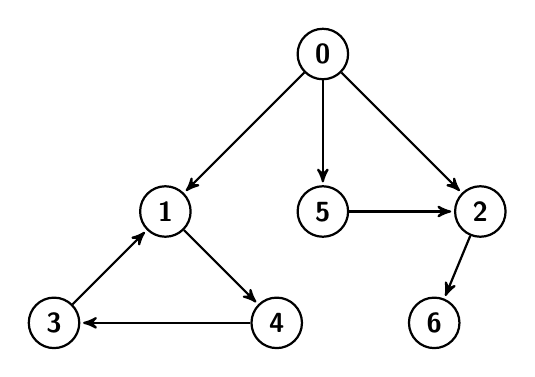
\begin{tikzpicture}[->,>=stealth',shorten >=1pt,auto,node distance=2cm,
  thick,main node/.style={circle,draw,font=\sffamily\bfseries}]
  
  \node[main node] (5) {5};
  \node[main node] (0) [above of=5] {0};
  \node[main node] (1) [left of=5] {1};
  \node[main node] (2) [right of=5] {2};
  \node[main node] (3) [below left of=1] {3};
  \node[main node] (4) [below right of=1] {4};
  \node[main node] (6) [right of=4] {6};

  \path[every node]
    (0) edge node {} (1)
        edge node {} (5)
        edge node {} (2)
    (1) edge node {} (4)
    (5) edge node {} (2)
    (4) edge node {} (3)
    (3) edge node {} (1)
    (2) edge node {} (6);
\end{tikzpicture}
\end{figure}
\end{problema}

\labtitle{Parcurgerea grafurilor. Grafuri ponderate\\ Drumuri de cost minim}{Parcurgerea grafurilor. Grafuri ponderate. Drumuri de cost minim}
\lab{9}
\begin{problema}[4][src/lab9_cityGraph.cpp]
  Presupunem că dispunem de o hartă cu $n$ orașe. Unele dintre acestea sunt unite prin șosele, acestea putând fi sau nu cu sens unic.
  Pentru fiecare șosea ce unește două orașe se cunoaște lungimea în kilometri.
  \begin{enumerate}
  \item[(a)] Un turist se află într-un oraș $s$ și vrea să ajungă cu mașina în orașul $f$.
    Se cere să se afle traseul de lungime minimă dintre cele două orașe.
  \item[(b)] Care sunt traseele de lungime minimă între $s$ și toate celelalte orașe?
  \item[(c)] Se cer traseele de lungime minimă între oricare două orașe de pe hartă.
  \end{enumerate}
\end{problema}

\labtitle{Arbori}{Arbori}
\lab{10}

\begin{problema}[7][src/lab10_adj.cpp]
  Fie arborele:
\begin{figure}[!h]
  \centering
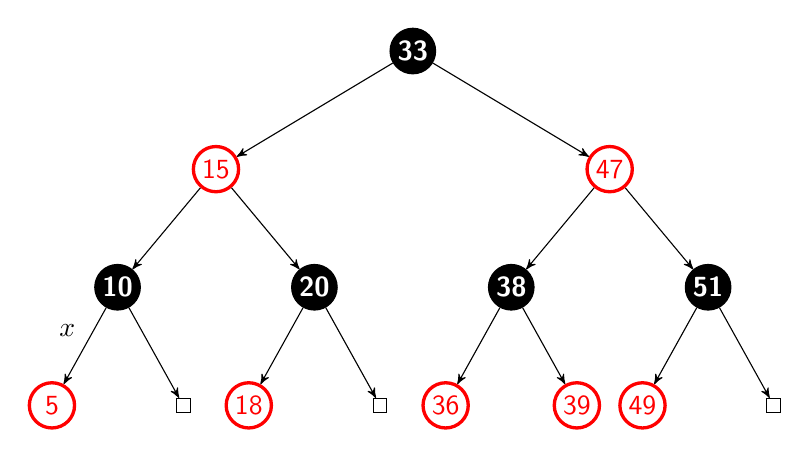
\begin{tikzpicture}[->,>=stealth',level/.style={sibling distance = 5cm/#1,
    level distance = 1.5cm}]
  \tikzset{
  treenode/.style = {align=center, inner sep=0pt, text centered,
    font=\sffamily},
  arn_n/.style = {treenode, circle, white, font=\sffamily\bfseries, draw=black,
    fill=black, text width=1.5em},% arbre rouge noir, noeud noir
  arn_r/.style = {treenode, circle, red, draw=red, 
    text width=1.5em, very thick},% arbre rouge noir, noeud rouge
  arn_x/.style = {treenode, rectangle, draw=black,
    minimum width=0.5em, minimum height=0.5em}% arbre rouge noir, nil
}
  \node [arn_n] {33}
    child{ node [arn_r] {15} 
            child{ node [arn_n] {10} 
            	child{ node [arn_r] {5} edge from parent node[above left]
                         {$x$}} %for a named pointer
							child{ node [arn_x] {}}
            }
            child{ node [arn_n] {20}
							child{ node [arn_r] {18}}
							child{ node [arn_x] {}}
            }                            
    }
    child{ node [arn_r] {47}
            child{ node [arn_n] {38} 
							child{ node [arn_r] {36}}
							child{ node [arn_r] {39}}
            }
            child{ node [arn_n] {51}
							child{ node [arn_r] {49}}
							child{ node [arn_x] {}}
            }
		}
        ;
\end{tikzpicture}
\end{figure}
\end{problema}



\end{document}
